\documentclass[11pt, fleqn]{article}

\usepackage{amsmath}
\usepackage{amssymb}
\usepackage{amsthm}
\usepackage{mathtools}
\usepackage{hyperref}
\usepackage{ulem}
\usepackage{enumitem}
\usepackage[left=0.75in, right=0.75in, bottom=0.75in, top=1.0in]{geometry}
\usepackage{floatrow}
\usepackage{graphicx}
\usepackage[export]{adjustbox}
\usepackage{sectsty}
\sectionfont{\centering}

\usepackage{multirow}
\usepackage{multicol}

\usepackage[dvipsnames]{xcolor}

\usepackage[perpage]{footmisc}

\usepackage{fancyhdr}
\pagestyle{fancy}
\fancyhf{}
\lhead{190100044}
\rhead{CS 252: Lab 5}
\renewcommand{\footrulewidth}{1.0pt}
\cfoot{Page \thepage}

\setlength{\parindent}{0em}

\title{\vspace{-4em}CS 252: Lab 5}
\author{Devansh Jain, 190100044}
\date{\today}

\begin{document}

% \pagenumbering{gobble}
\maketitle
\tableofcontents
\thispagestyle{empty}
\setcounter{page}{0}


\newpage 
\section*{Question 1}
\addcontentsline{toc}{section}{Question 1}
\setcounter{equation}{0}

\subsection*{a.}
\addcontentsline{toc}{subsection}{a.}

For default parameters (\texttt{dataRate} = 10.0Mbps),\\

Throughput for Flow 1 (Node n1 $\rightarrow$ Node n0): \\
9.71408 Mbps (RTS/CTS disabled), 10.1113 Mbps (RTS/CTS enabled) \\

Throughput for Flow 2 (Node n2 $\rightarrow$ Node n0): \\
9.37797 Mbps (RTS/CTS disabled), 10.096 Mbps (RTS/CTS enabled) \\

Total Channel Throughput: \\
19.0921 Mbps (RTS/CTS disabled), 20.2073 Mbps (RTS/CTS enabled) \\

\subsection*{b.}
\addcontentsline{toc}{subsection}{b.}

Channel data rate is 54 Mbps.

\begin{figure}[H]
    \centering
    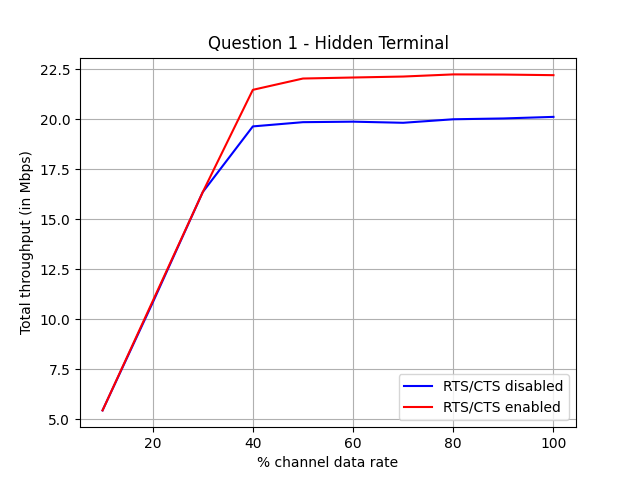
\includegraphics{q1.png}
\end{figure}

\begin{table}[H]
    \centering
    \begin{tabular}{||c|c||c|c||}
         \hline
         \multirow{2}{*}{Total Data Rate Offered} & \multirow{2}{*}{\texttt{dataRate}} & \multicolumn{2}{c||}{Total Throughput} \\
         & & RTS/CTS disabled & RTS/CTS enabled \\
         \hline % 10
         10\% of channel date rate & 2.7Mbps & 5.45414 Mbps & 5.45414 Mbps \\
         \hline % 20
         20\% of channel date rate & 5.4Mbps & 10.8344 Mbps & 10.9108 Mbps \\
         \hline % 30
         30\% of channel date rate & 8.1Mbps & 16.3675 Mbps & 16.3675 Mbps \\
         \hline % 40
         40\% of channel date rate & 10.8Mbps & 19.6522 Mbps & 21.4805 Mbps \\
         \hline % 50
         50\% of channel date rate & 13.5Mbps & 19.8636 Mbps & 22.0457 Mbps \\
         \hline % 60
         60\% of channel date rate & 16.2Mbps & 19.889 Mbps & 22.0967 Mbps \\
         \hline % 70
         70\% of channel date rate & 18.9Mbps & 19.833 Mbps & 22.145 Mbps \\
         \hline % 80
         80\% of channel date rate & 21.6Mbps & 20.0087 Mbps & 22.252 Mbps \\
         \hline % 90
         90\% of channel date rate & 24.3Mbps & 20.0495 Mbps & 22.2444 Mbps \\
         \hline % 100
         100\% of channel date rate & 27.0Mbps & 20.1284 Mbps & 22.2138 Mbps \\
         \hline         
    \end{tabular}
\end{table}

We can see that Total throughput increases with Offered Load and almost flattens to a constant value by the end. \\
We also see that RTS/CTS disabled network has less maximum throughput than RTS/CTS enabled network. \\

\subsection*{c.}
\addcontentsline{toc}{subsection}{c.}
Only Flow 1 (Node n1 $\rightarrow$ Node n0) \\
RTS/CTS disabled: Total throughput saturates at 25.6182 Mbps for \texttt{dataRate} = 35 Mbps. \\
RTS/CTS enabled: Total throughput saturates at 22.6339 Mbps for \texttt{dataRate} = 24 Mbps. \\

We can see that Total throughput increases with Offered Load and almost flattens to a constant value by the end. \\
We also see that RTS/CTS disabled network has more maximum throughput than RTS/CTS enabled network. \\

\subsection*{d.}
\addcontentsline{toc}{subsection}{d.}

\begin{itemize}
    \item Total throughput is less than total data rate offered in all cases.
    \item We can see that Total throughput increases with Offered Load and almost flattens to a constant value by the end, both for two source and one source
    \item We also see that RTS/CTS disabled network has less maximum throughput than RTS/CTS enabled network when we have two sources but has more maximum throughput when we have only one source.
    \item We reach saturation for both cases when total data rate offered is about 40\% of channel data rate.
\end{itemize}

\newpage
\section*{Question 2}
\addcontentsline{toc}{section}{Question 2}
\setcounter{equation}{0}

\subsection*{a.}
\addcontentsline{toc}{subsection}{a.}

Channel data rate is 54 Mbps.

\begin{figure}[H]
    \centering
    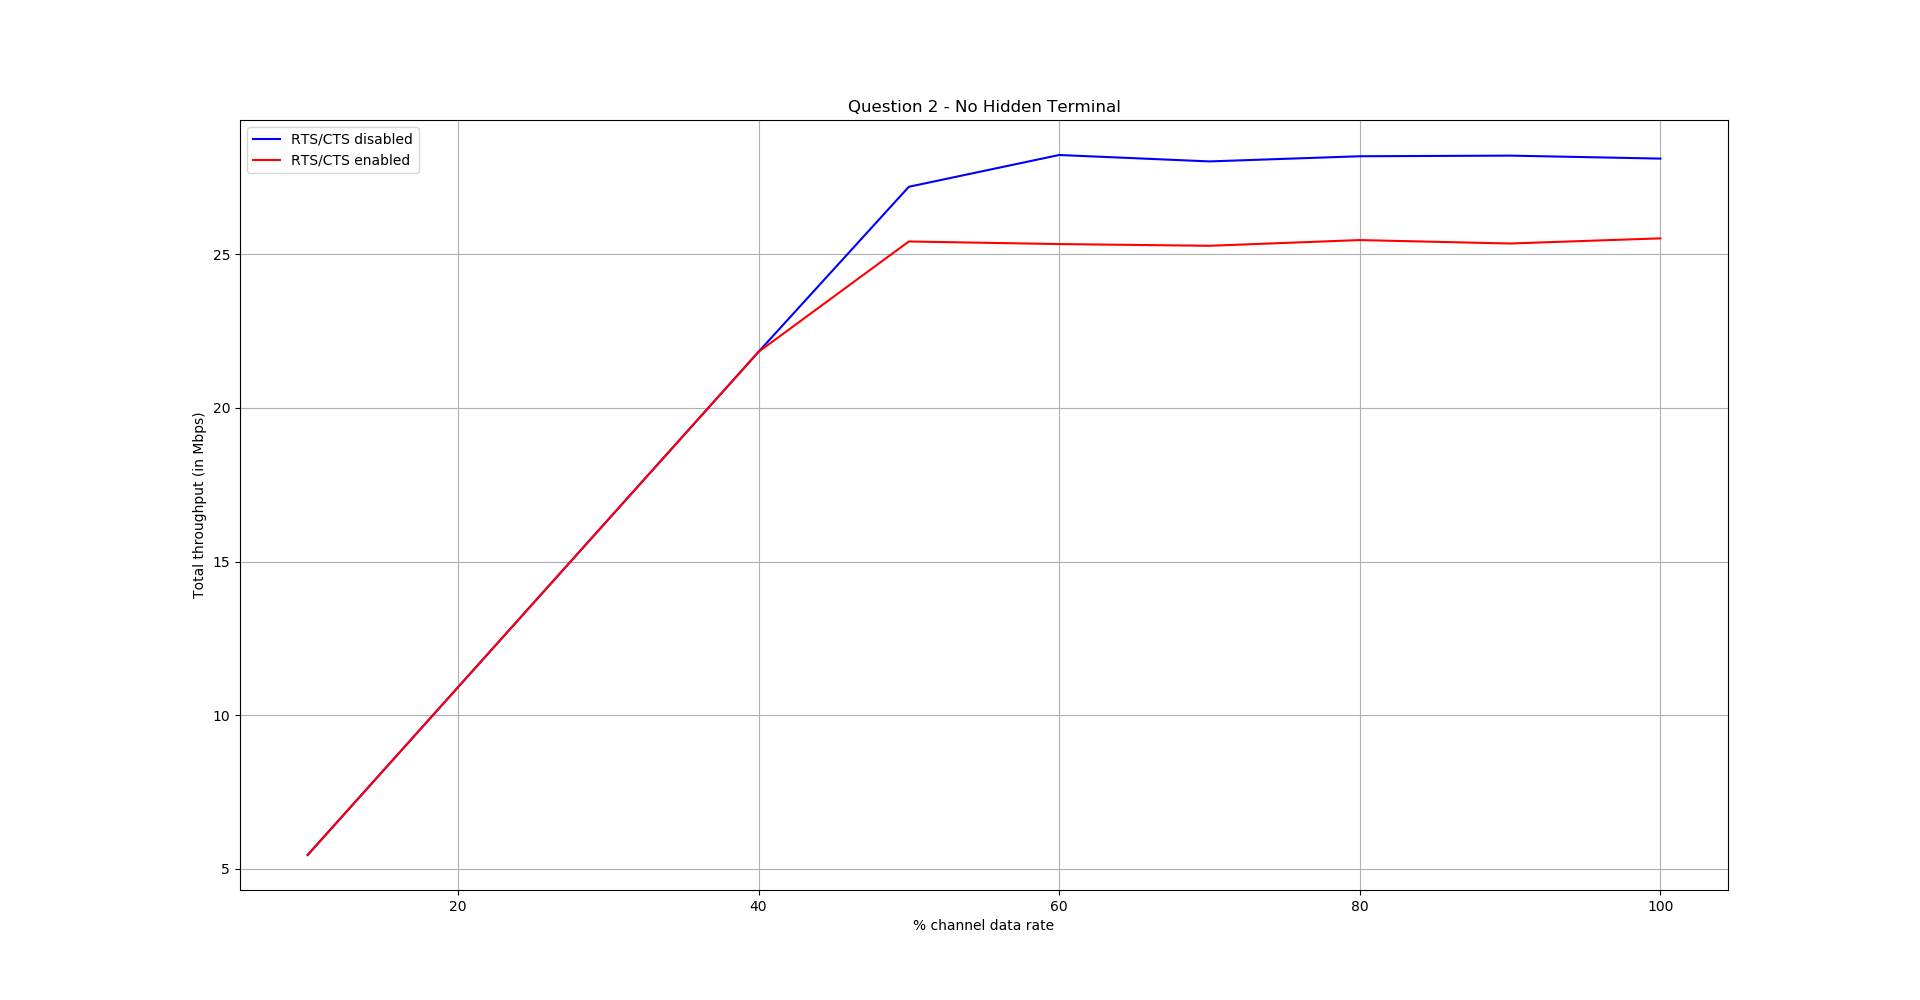
\includegraphics{q2.png}
\end{figure}

\begin{table}[H]
    \centering
    \begin{tabular}{||c|c||c|c||}
         \hline
         \multirow{2}{*}{Total Data Rate Offered} & \multirow{2}{*}{\texttt{dataRate}} & \multicolumn{2}{c||}{Total Throughput} \\
         & & RTS/CTS disabled & RTS/CTS enabled \\
         \hline % 10
         10\% of channel date rate & 2.7Mbps & 5.45414 Mbps & 5.45414 Mbps \\
         \hline % 20
         20\% of channel date rate & 5.4Mbps & 10.9108 Mbps & 10.9108 Mbps \\
         \hline % 30
         30\% of channel date rate & 8.1Mbps & 16.3675 Mbps & 16.3675 Mbps \\
         \hline % 40
         40\% of channel date rate & 10.8Mbps & 21.8242 Mbps & 21.8242 Mbps \\
         \hline % 50
         50\% of channel date rate & 13.5Mbps & 27.1943 Mbps & 25.4145 Mbps \\
         \hline % 60
         60\% of channel date rate & 16.2Mbps & 28.2281 Mbps & 25.3305 Mbps \\
         \hline % 70
         70\% of channel date rate & 18.9Mbps & 28.0193 Mbps & 25.2744 Mbps \\
         \hline % 80
         80\% of channel date rate & 21.6Mbps & 28.1874 Mbps & 25.4603 Mbps \\
         \hline % 90
         90\% of channel date rate & 24.3Mbps & 28.2078 Mbps & 25.3483 Mbps \\
         \hline % 100
         100\% of channel date rate & 27.0Mbps & 28.111 Mbps & 25.5163 Mbps \\
         \hline         
    \end{tabular}
\end{table}

We can see that Total throughput increases with Offered Load and almost flattens to a constant value by the end. \\
We also see that RTS/CTS disabled network has more maximum throughput than RTS/CTS enabled network. \\

\subsection*{b.}
\addcontentsline{toc}{subsection}{b.}

\begin{itemize}
    \item Total throughput is less than total data rate offered in all cases.
    \item We can see that Total throughput increases with Offered Load and almost flattens to a constant value by the end, both for two source and one source
    \item We also see that RTS/CTS disabled network has more maximum throughput than RTS/CTS enabled network.
    \item We reach saturation for both cases when total data rate offered is about 50\% of channel data rate.
    \item The saturation level as compared to Question 1 (where a hidden terminal pair was present) is more for both cases.
\end{itemize}

\newpage 
\section*{Question 3}
\addcontentsline{toc}{section}{Question 3}
\setcounter{equation}{0}

\subsection*{a.}
\addcontentsline{toc}{subsection}{a.}

For default parameters (\texttt{dataRate} = 10.0Mbps),\\

Throughput for Flow 1 (Node A1 $\rightarrow$ Node A2): 10.1088 Mbps (RTS/CTS enabled) \\
Throughput for Flow 2 (Node B1 $\rightarrow$ Node B2): 9.52565 Mbps (RTS/CTS enabled) \\
Throughput for Flow 3 (Node C1 $\rightarrow$ Node C2): 10.0807 Mbps (RTS/CTS enabled) \\

Total Channel Throughput: 29.7152 Mbps (RTS/CTS enabled) \\

\subsection*{b.}
\addcontentsline{toc}{subsection}{b.}

Channel data rate is 54 Mbps.

\begin{figure}[H]
    \centering
    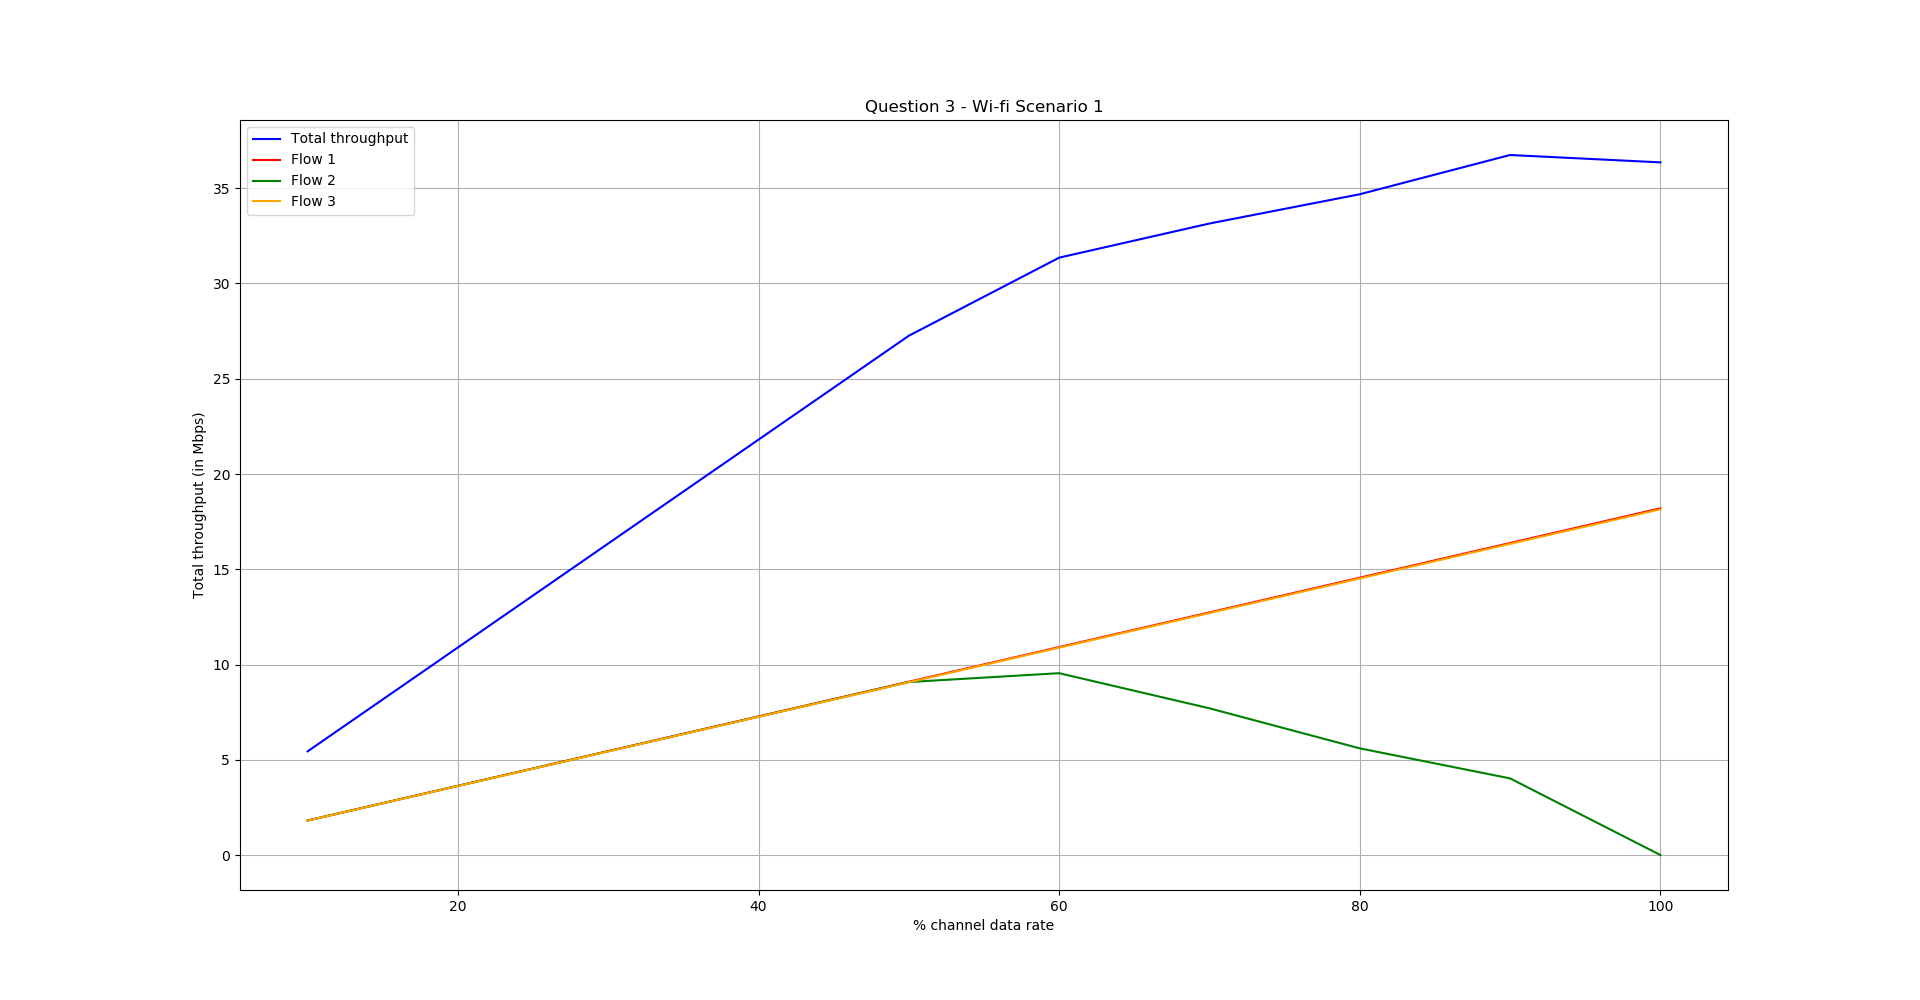
\includegraphics{q3.png}
\end{figure}

\begin{table}[H]
    \centering
    \begin{tabular}{||c|c||c||}
         \hline
         Total Data Rate Offered & \texttt{dataRate} & Total Throughput \\
         \hline % 10
         10\% of channel date rate & 1.8Mbps & 5.44651 Mbps \\
         \hline % 20
         20\% of channel date rate & 3.6Mbps & 10.9006 Mbps \\
         \hline % 30
         30\% of channel date rate & 5.4Mbps & 16.3548 Mbps \\
         \hline % 40
         40\% of channel date rate & 7.2Mbps & 21.8064 Mbps \\
         \hline % 50
         50\% of channel date rate & 9.0Mbps & 27.258 Mbps \\
         \hline % 60
         60\% of channel date rate & 10.8Mbps & 31.2837 Mbps \\
         \hline % 70
         70\% of channel date rate & 12.6Mbps & 33.145 Mbps \\
         \hline % 80
         80\% of channel date rate & 14.4Mbps & 34.8485 Mbps \\
         \hline % 90
         90\% of channel date rate & 16.2Mbps & 36.4195 Mbps \\
         \hline % 100
         100\% of channel date rate & 18.0Mbps & 36.3559 Mbps \\
         \hline         
    \end{tabular}
\end{table}

We can see that Total throughput increases with Offered Load and almost flattens to a constant value by the end. \\

\subsection*{c.}
\addcontentsline{toc}{subsection}{c.}

\begin{itemize}
    \item Total throughput is less than total data rate offered.
    \item We can see that Total throughput increases with Offered Load and almost flattens to a constant value by the end.
    \item We reach saturation when total data rate offered is about 90\% of channel data rate.
    \item Comparing between the flows, we can see that Throughputs of Flow 1 and Flow 3 are almost equal. This can be seen easily by symmetry.
    \item Throughputs of Flow 1 and Flow 3 are more than Flow 2. If we take different cases of who sends first among A1. B1, C1.
\end{itemize}

\newpage 
\section*{Question 4}
\addcontentsline{toc}{section}{Question 4}
\setcounter{equation}{0}

\subsection*{a.}
\addcontentsline{toc}{subsection}{a.}

For default parameters (\texttt{dataRate} = 10.0Mbps),\\

Throughput for Flow 1 (Node A $\rightarrow$ Node B): 7.79927 Mbps (RTS/CTS enabled) \\
Throughput for Flow 2 (Node C $\rightarrow$ Node D): 10.096 Mbps (RTS/CTS enabled) \\

Total Channel Throughput: 17.8953 Mbps (RTS/CTS enabled) \\

\subsection*{b.}
\addcontentsline{toc}{subsection}{b.}

Channel data rate is 54 Mbps.

\begin{figure}[H]
    \centering
    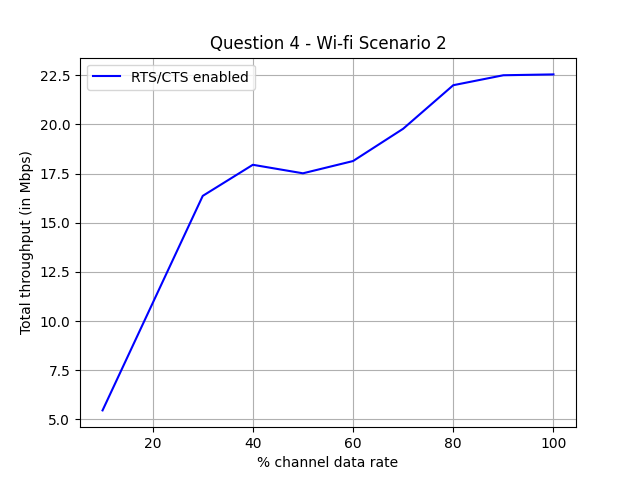
\includegraphics{q4.png}
\end{figure}

\begin{table}[H]
    \centering
    \begin{tabular}{||c|c||c||}
         \hline
         Total Data Rate Offered & \texttt{dataRate} & Total Throughput \\
         \hline % 10
         10\% of channel date rate & 2.7Mbps & 5.45414 Mbps \\
         \hline % 20
         20\% of channel date rate & 5.4Mbps & 10.9108 Mbps \\
         \hline % 30
         30\% of channel date rate & 8.1Mbps & 16.3675 Mbps \\
         \hline % 40
         40\% of channel date rate & 10.8Mbps & 17.9462 Mbps \\
         \hline % 50
         50\% of channel date rate & 13.5Mbps & 17.5159 Mbps \\
         \hline % 60
         60\% of channel date rate & 16.2Mbps & 18.1397 Mbps \\
         \hline % 70
         70\% of channel date rate & 18.9Mbps & 19.7821 Mbps \\
         \hline % 80
         80\% of channel date rate & 21.6Mbps & 21.9974 Mbps \\
         \hline % 90
         90\% of channel date rate & 24.3Mbps & 22.5041 Mbps \\
         \hline % 100
         100\% of channel date rate & 27.0Mbps & 22.5474 Mbps \\
         \hline         
    \end{tabular}
\end{table}

We can see that Total throughput increases with Offered Load and almost flattens to a constant value by the end with a minor dip in middle. \\

\subsection*{c.}
\addcontentsline{toc}{subsection}{c.}


\end{document}
